\setlength{\headheight}{30pt}
% ****** Start of file apssamp.tex ******
%
%   This file is part of the APS files in the REVTeX 4.1 distribution.
%   Version 4.1r of REVTeX, August 2010
%
%   Copyright (c) 2009, 2010 The American Physical Society.
%
%   See the REVTeX 4 README file for restrictions and more information.
%
% TeX'ing this file requires that you have AMS-LaTeX 2.0 installed
% as well as the rest of the prerequisites for REVTeX 4.1
%
% See the REVTeX 4 README file
% It also requires running BibTeX. The commands are as follows:
%
%  1)  latex apssamp.tex
%  2)  bibtex apssamp
%  3)  latex apssamp.tex
%  4)  latex apssamp.tex
%
\documentclass[%
reprint,
%superscriptaddress,
%groupedaddress,
%unsortedaddress,
%runinaddress,
%frontmatterverbose, 
%preprint,
%showpacs,preprintnumbers,
%nofootinbib,
%nobibnotes,
%bibnotes,
amsmath,amssymb,
aps,
12pt
%pra,
%prb,
%rmp,
%prstab,
%prstper,
%floatfix,
]{revtex4-1}


\usepackage{graphicx}% Include figure files
\usepackage{dcolumn}% Align table columns on decimal point
\usepackage{bm}% bold math
\usepackage{hyperref}% add hypertext capabilities
\usepackage[mathlines]{lineno}% Enable numbering of text and display math
\usepackage{amsmath} % assumes amsmath package installed
\usepackage{amssymb}  % assumes amsmath package installed

\usepackage{epsfig} % for postscript graphics files
\usepackage{mathptmx} % assumes new font selection scheme installed
\usepackage{times} % assumes new font selection scheme installed
\usepackage{ucs}
\usepackage[utf8x]{inputenc}
\usepackage[portuguese,brazil]{babel} % [english]
\usepackage[T1]{fontenc}
\usepackage{indentfirst}
\usepackage{amsfonts,amssymb,amsmath,amsthm}
\usepackage{ae} % font "amost european"
\usepackage{graphicx} % add [draft] para compilar rápido (quadrado branco no lugar da figura)
\usepackage{color}
\usepackage{wrapfig}
\usepackage{braket}
\raggedbottom % prevents LaTeX from adding vertical white space in strange places on pages that it cannot fill properly
\usepackage[top=3cm, left=2.1cm, right=2.1cm, bottom=2.5cm]{geometry}
\pagestyle{headings}

%---- Espaçamento entre as linhas ----

\newcommand{\blst}{1.2} %{1.15}
\renewcommand{\baselinestretch}{\blst}

\raggedbottom

%\linenumbers\relax % Commence numbering lines

%\usepackage[showframe,%Uncomment any one of the following lines to test 
%%scale=0.7, marginratio={1:1, 2:3}, ignoreall,% default settings
%%text={7in,10in},centering,
%%margin=1.5in,
%%total={6.5in,8.75in}, top=1.2in, left=0.9in, includefoot,
%%height=10in,a5paper,hmargin={3cm,0.8in},
%]{geometry}
\def\bibsection{\section{Bibliography}} 
\begin{document}
	
	\preprint{APS/123-QED}
	
	\title{Sistemas de Discos Rígidos}% Force line breaks with \\
	
	\author{Diego Oliveira}
	\affiliation {Instituto de Física, Universidade Estadual de Campinas-Unicamp, Campinas, São Paulo, 13083-859, Brasil}
	\email{dso@ifi.unicamp.br}
	
	%\date{\today}% It is always \today, today,
	%  but any date may be explicitly specified
	
	\begin{abstract}
	Neste trabalho tentaremos observar a transição de fase líquido-solido utilizando sistemas de discos rígidos. O sistema foi simulado utilizando três métodos diferentes: Dinâmica Molecular, Monte Carlo Amostragem-Direta e Monte Carlo Amostragem-Cadeia de Markov. Ao simularmos o ultimo método com condições periódicas de contorno, observamos uma transição de fase líquido-solido.
	\end{abstract}
	
	%\pacs{Valid PACS appear here}% PACS, the Physics and Astronomy
	% Classification Scheme.
	%\keywords{Semiconductor lasers, quantum wells}%Use showkeys class option if keyword
	%display desired
\maketitle


\maketitle
\renewcommand{\thesection}{\arabic{section}}
\renewcommand{\thesubsection}{\thesection.\arabic{subsection}}
\renewcommand{\thesubsubsection}{\thesubsection.\arabic{subsubsection}}

% Fix references
\makeatletter
\renewcommand{\p@subsection}{}
\renewcommand{\p@subsubsection}{}
\makeatother
%\tableofcontents
	
\section{Introdução}
A simulação de sistemas físicos vem se tornando cada vez mais fundamental na compreensão de sistemas reais, pois com ela podemos predizer propriedades de forma rápida e simples de modelos teóricos complexos, além de respaldar experimentos.

Neste trabalho tentaremos observar a transição de fase líquido-solido utilizando sistemas de discos rígidos (não permite sobreposição). Os sistemas de discos rígidos desempenharam um papel fundamental na gênesis da mecânica estatística e computacional. Desde os primórdios da computação na década de 50, este modelo tem estimulado o desenvolvimento de algoritmos tanto para a integração numérica explicita das equações de Newton (\textbf{Dinâmica Molecular}), como para métodos estocásticos (\textbf{Monte Carlo}). Utilizaremos estes algoritmos para introduzir princípios fundamentais da mecânica estatística, como o principio da equiprobabilidade e a distribuição de Bolztmann. Também introduzimos o conceito de condições periódicas de contorno, o que foi essencial para a obtenção de nossos resultados.

Na próxima seção apresentaremos o sistema e suas grandezas de interesse; em seguida mostraremos algumas abordagens na solução do problema, utilizando simulações de \textit{Dinâmica Molecular}, \textit{Método de  Monte Carlo-Amostragem Direta} e \textit{Método de  Monte Carlo-Cadeia de Markov}. Por fim, apresentaremos os resultados obtidos e conclusões.

\section{O sistema de discos rígidos}
 Neste sistema iremos considerar $ N $ discos rígidos idênticos de raio  $ \sigma $  em uma caixa quadrada de dimensões $ L \times L $ (figura \ref{sistema}). Controlaremos o sistema variando sua densidade, que é dada por $ \eta = N \pi {\sigma}^2/L^2 $.
 
 \begin{figure}[!h]
 	\centering
 	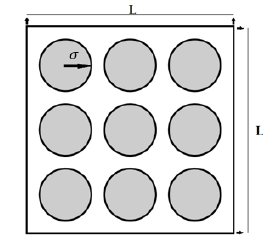
\includegraphics[scale=0.5]{sistema.png}
 	\caption{Representação do sistema de discos rígidos com  $ N = 9 $.
 		%\caption{Hypothetical absorption spectrum for a typical semiconductor as a function of photon energy
 		\label{sistema}}
 \end{figure}
 
 O potencial de interação entre os discos rígidos é dado por
 
 
\begin{equation}
U_{12}(r) = \left \{ \begin{matrix} + \infty, & \mbox{$ r < 2\sigma $  } \\ 0, & \mbox{$ r \geq 2\sigma $} \end{matrix} \right.,
\end{equation}

onde $ r = |\textbf{r}_1 - \textbf{r}_2|$  é a distância entre um par de discos e $ \sigma $ é o raio do disco.

 

 	

 
	

\section{Dinâmica Molecular}
A Dinâmica Molecular é uma ferramenta computacional que tem por objetivo principal o estudo do comportamento de um sistema de partículas em função do tempo.

Este conceito foi introduzido por Alder e Wainwright em 1957 no estudos de interações entre esferas rígidas que interagem através de colisões perfeitas\cite{alder}.

Classicamente, em Dinâmica Molecular, as sucessivas configurações do sistema são geradas pela integração das equações de movimento de Newton. O resultado é uma trajetória que especifica como as posições e velocidades das partículas dos sistema variam com o tempo (figura \ref{dm1}).

\begin{figure}[!h]
	\centering
	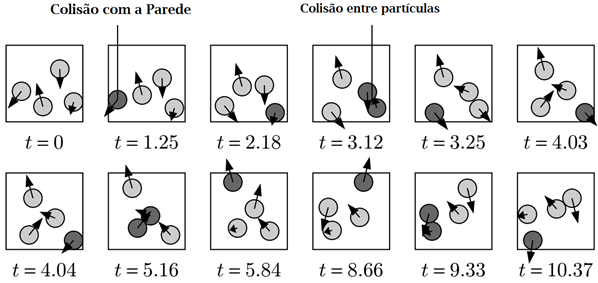
\includegraphics[scale=0.52]{dm1.png}
	\caption{Representação da evolução temporal de um sistema de discos rígidos.
		\label{dm1}}
\end{figure}

No sistema estudado, todos os discos se propagam livremente com velocidade constante até que ocorra uma colisão (única forma de interação), onde todas as colisões são elásticas; isto é, momento linear e energia cinéticas são conservados. Este sistema possui dois tipos de colisão: partícula-partícula (caso a distância entre partículas seja menor que $ 2\sigma $), e partícula-parede (figura \ref{dm1}). 

Podemos escrever um algoritmo baseado nos eventos que ocorrem no interior da caixa da seguinte forma:

\textbf{1.} Introduzir configuração inicial dos discos (posições e velocidades).

\textbf{2.} Determinar o tempo de colisão com a parede para todas as partículas via equações de newton.

\textbf{3.} Determinar o tempo de colisão entre partículas para todas as partículas via equações de newton.

\textbf{4.} Para cada partícula, escolher o menor tempo de colisão entre os passos 1 e 2.

\textbf{5.} Partícula se propaga livremente até que chegue o tempo determinado no passo 4.

\textbf{6.} Determinar as novas posições e velocidades via cálculos de conservação.

\textbf{7.} Retornamos ao passo 1 com as novas velocidades e posições.


Implementando o algoritmo acima obtemos os resultados mostrado na figura \ref{dm2}.

\begin{figure}[!h]
	\centering
	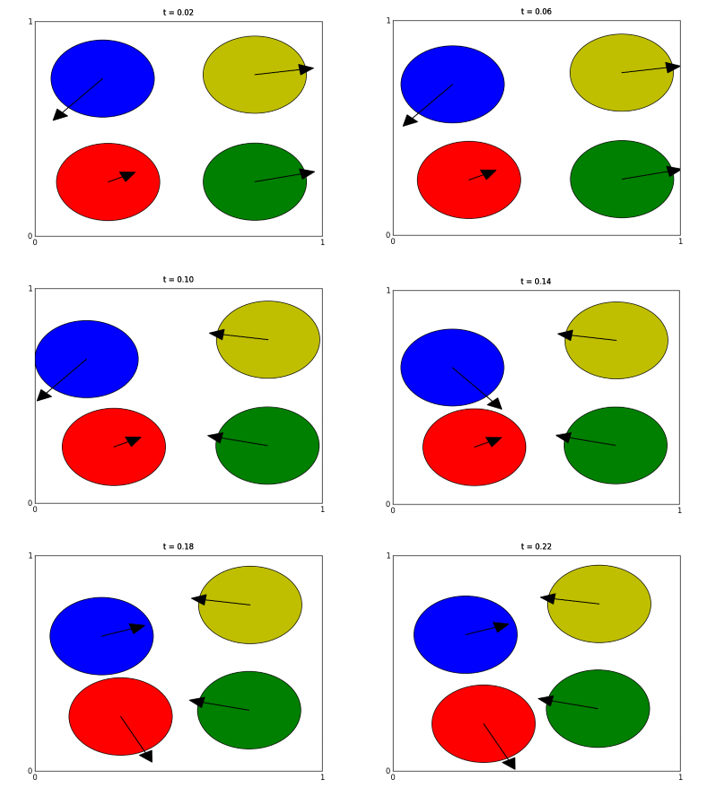
\includegraphics[scale=0.15]{dm2.png}
	\caption{Simulação de Dinâmica Molecular para um sistema de discos rígidos.
		\label{dm2}}
\end{figure}



Apesar da simulação por Dinâmica Molecular nos fornecer uma descrição detalhada do sistema (figura \ref{dm2}), ela se mostrou ineficiente pois seu custo computacional e a complexidade em sua implementação aumentam muito com a adição de novos discos. 


\section{Monte Carlo}

O método de Monte Carlo é uma alternativa para contornarmos o problema encontrado na simulação por Dinâmica Molecular, por ser computacionalmente mais barato e de simples implementação.

A simulação de Monte Carlo é um método numérico que nasceu em 1949 com trabalhos de John Von Neumann e Stanislav Ulam, a fim de avaliar soluções para alguns problemas matemáticos (\cite{newman}). Em princípio, o método de Monte Carlo não foi feito para resolver problemas na Física, mas para calcular integrais. No entanto, em 1953, Metropolis e outros colaboradores aperfeiçoaram o método como um instrumento que encontra uso em mecânica estatística (\cite{metrop}). Atualmente, com o avanço dos computadores e o desenvolvimento de poderosos algoritmos, o método de Monte Carlo tornou-se uma importante ferramenta em todos os campos da ciência.

 Para aplicarmos este método ao nosso sistema, primeiramente precisamos saber qual distribuição de probabilidade devemos amostrar, ou seja, com qual frequência uma certa configuração \textbf{a} aparece durante uma amostragem suficientemente grande. 

Nosso sistema é fundamentado na mecânica estatística de Boltzmann e segue o principio da equiprobabilidade (figura \ref{mc}), onde duas configurações \textbf{a} e \textbf{b} possuem a mesma probabilidade de aparecer.

\begin{equation}
\pi(a) = \pi(b)
\end{equation}




\begin{figure}[!h]
	\centering
	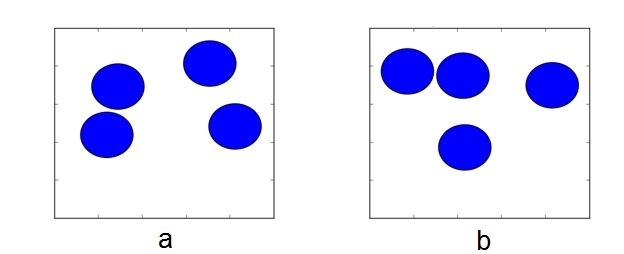
\includegraphics[scale=0.5]{mc.png}
	\caption{Representação do principio da equiprobabilidade, onde os estados a e b possuem a mesma probabilidade de serem amostrados.
		\label{mc}}
\end{figure}	




\subsection{Amostragem Direta}
 
Seguindo o principio da equiprobabilidade, todas as configurações devem ser geradas com o mesmo peso estatístico. Isso pode ser colocado em prática gerando todos os tipos de configurações, válidas e inválidas, com o mesma probabilidade, onde aceitamos as configurações válidas e rejeitamos as inválidas, ou seja:

\begin{equation}
\pi(x_1,x_2 ,...,x_N) = \left \{ \begin{matrix} 1, & \mbox{conf. válida} \\ 0, & \mbox{conf. inválida} \end{matrix} \right.
\end{equation}

Colocando isso em forma de um algoritmo, temos:

\textbf{1.} Gerar uma configuração aleatória dos discos no interior da caixa.

\textbf{2.} Checar se ocorre sobreposição entre os discos ou a caixa.

\textbf{3.} Se ocorrer sobreposição, a configuração é recusada e retornamos ao passo 1.

\textbf{4.} Caso não ocorra sobreposição, a configuração é aceita e adicionada à nossa estatística, e então retornamos para o passo 1.

A figura \ref{mcd} mostra uma ilustração do algoritmo acima.

\begin{figure}[!h]
	\centering
	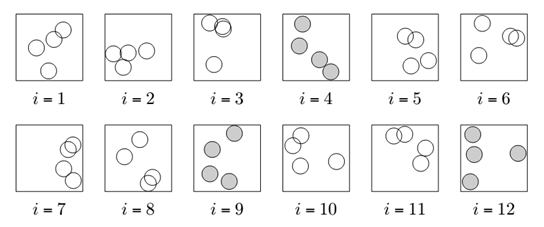
\includegraphics[scale=0.6]{mcd.png}
	\caption{Ilustração do algoritmo de amostragem direta, onde as configurações com os discos não preenchidos possuem sobreposição e são recusadas, enquanto as configurações com discos preenchidos não possuem sobreposição e são aceitas.
		\label{mcd}}
\end{figure}

Implementando o algoritmo acima, obtemos os resultados mostrados nas figuras \ref{mcd1}, \ref{mcd2}, \ref{mcd3} e \ref{mcd4}.
 

\begin{figure}[!h]
	\centering
	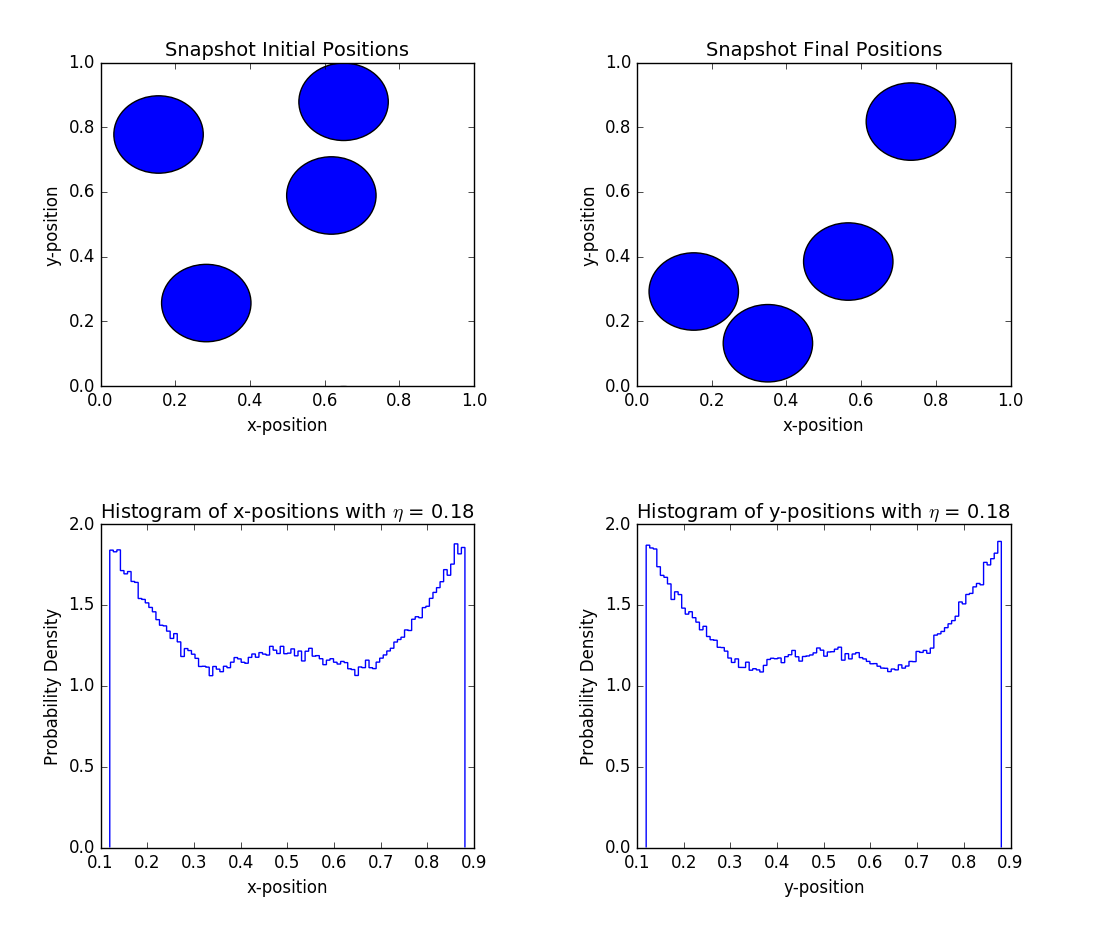
\includegraphics[scale=0.28]{mcd1.png}
	\caption{Resultado para uma simulação com rotina de $ 10^5 $ e $ \eta = 0.18 $ temos um tempo total de simulação de 4 segundos.
	\label{mcd1}}
\end{figure}
\begin{figure}[!h]
	\centering
	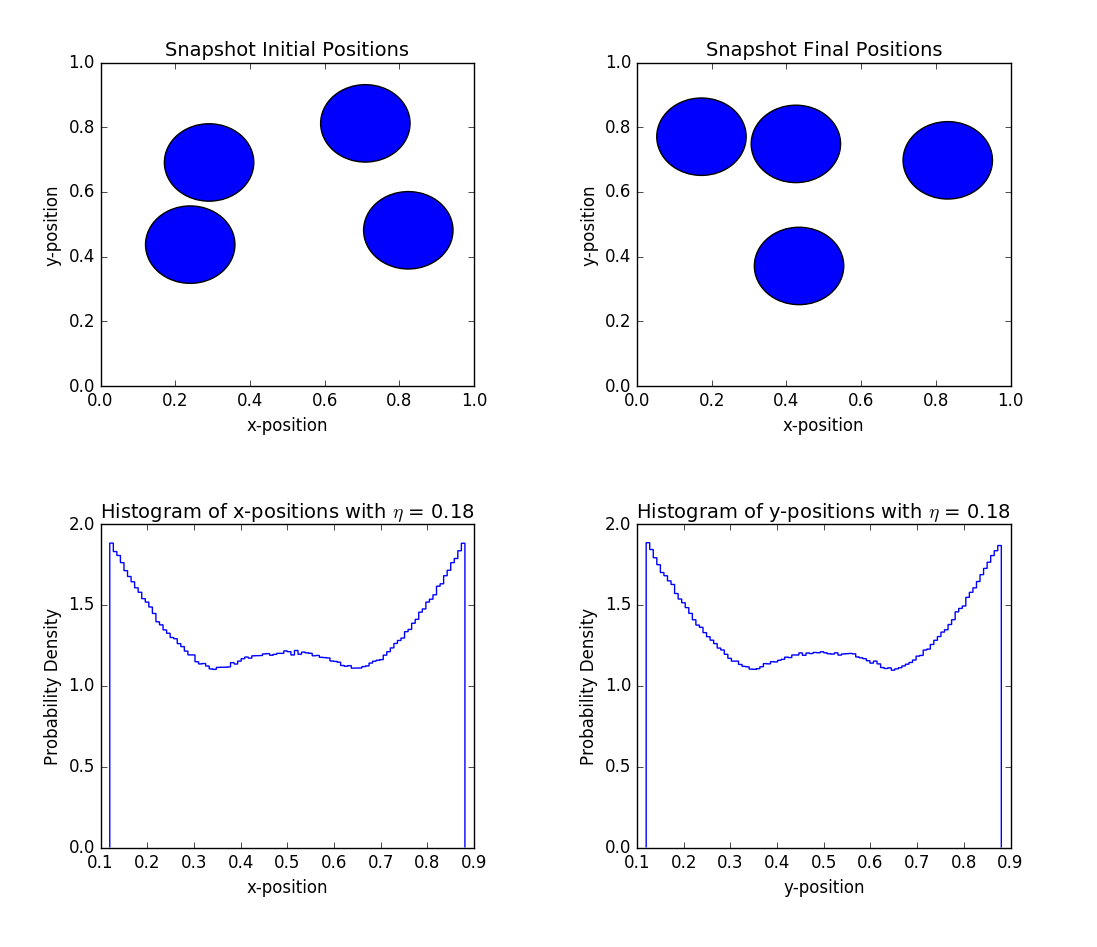
\includegraphics[scale=0.28]{mcd2.png}
	\caption{Resultado para uma simulação com rotina de $ 10^6 $ e $ \eta = 0.18 $ temos um tempo total de simulação de 45 segundos.
		\label{mcd2}}
\end{figure}
\begin{figure}[!h]
	\centering
	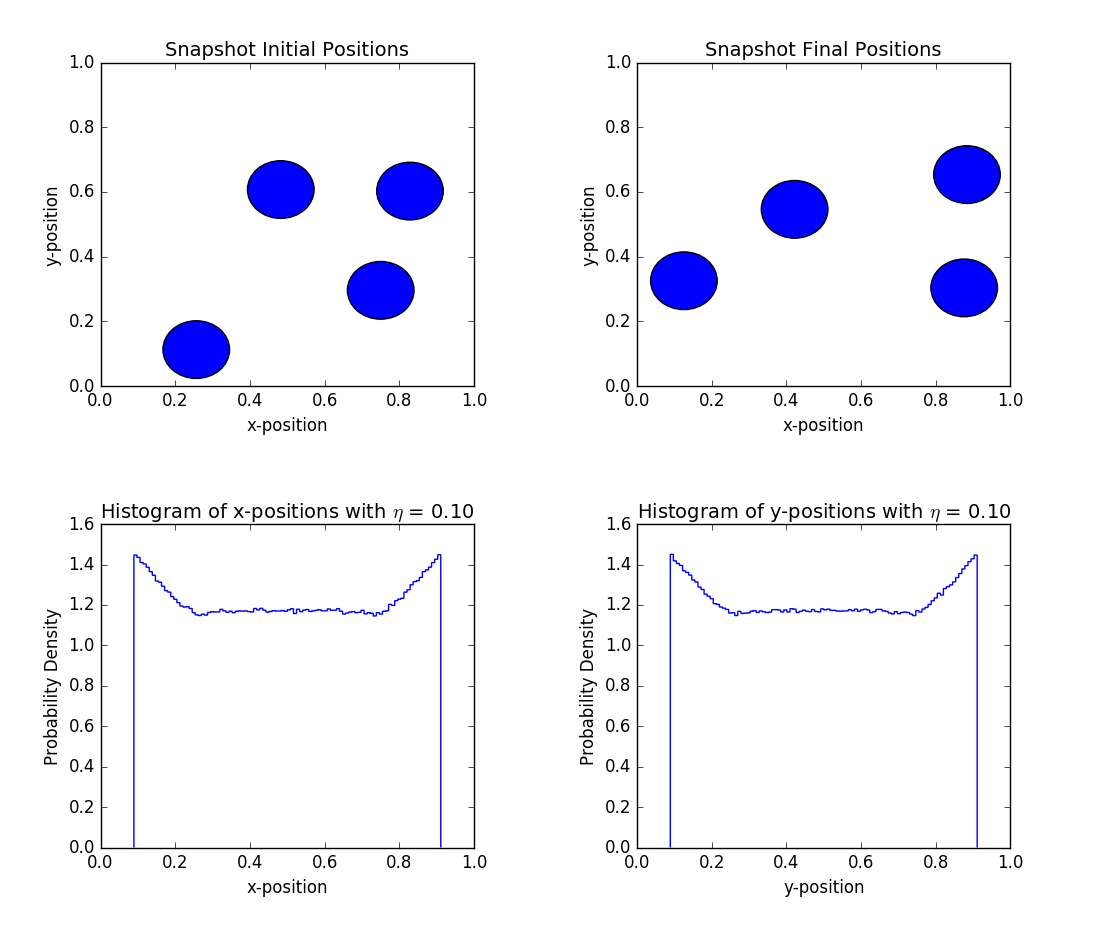
\includegraphics[scale=0.28]{mcd3.png}
	\caption{Resultado para uma simulação com rotina de $ 10^6 $ e $ \eta = 0.10 $ temos um tempo total de simulação de 22 segundos.
		\label{mcd3}}
\end{figure}
\clearpage
\begin{figure}[!h]
	\centering
	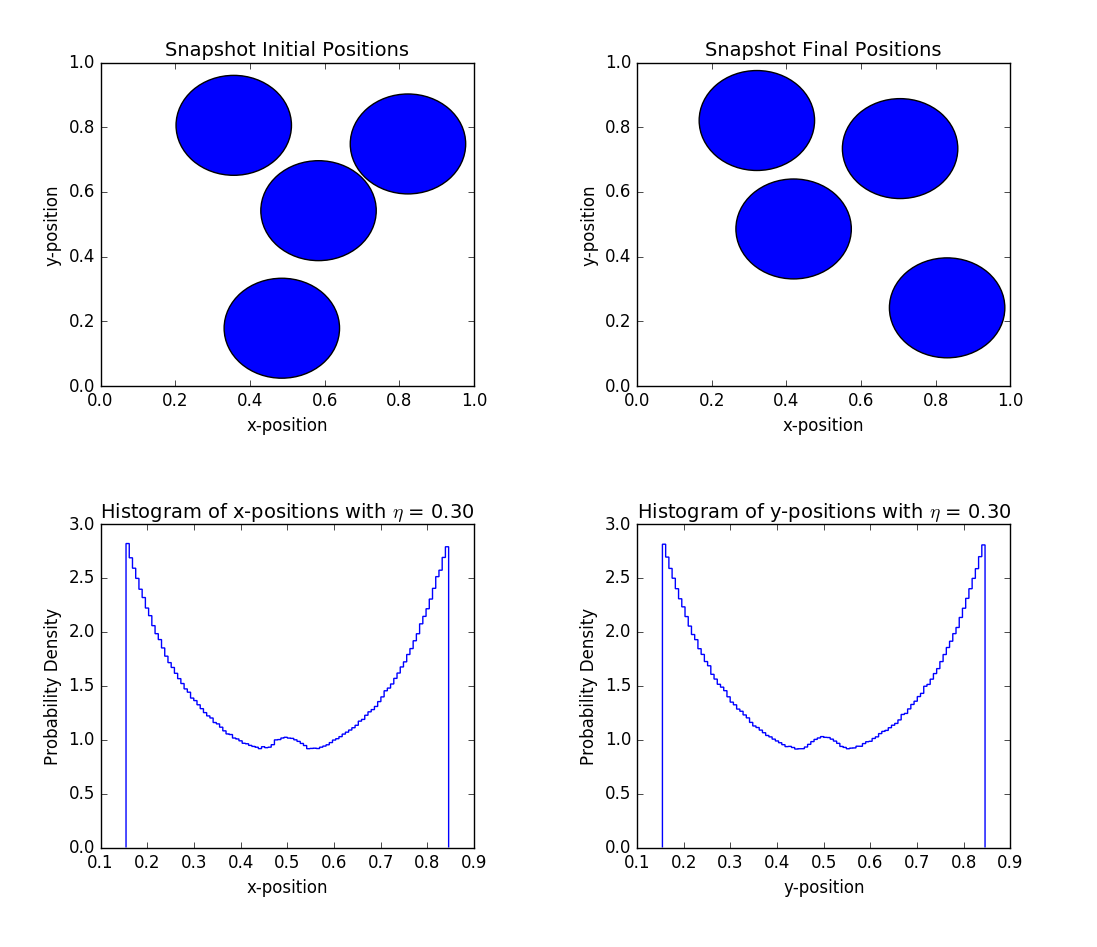
\includegraphics[scale=0.28]{mcd4.png}
	\caption{Resultado para uma simulação com rotina de $ 10^6 $ e $ \eta = 0.30 $ temos um tempo total de simulação de 257 segundos.
		\label{mcd4}}
\end{figure}


Ao compararmos os resultados das figuras \ref{mcd1} e \ref{mcd2}, observamos um aumento de aproximadamente 11 vezes no tempo de simulação ao aumentarmos a rotina em uma ordem de grandeza. Comparando os resultados das figuras \ref{mcd2}, \ref{mcd3} e \ref{mcd4}, observamos um grande aumento no tempo de simulação conforme aumentamos o valor de $ \eta $.
Em uma simulação com $ N = 16 $, $ \eta = 0.3 $ e $ 10^6 $ tentativas obtemos apenas 8 configurações válidas. Isto ilustra a ineficiência da amostragem direta, pois ao aumentarmos os valores de $ \eta $ ou $ N $, o nível de rejeição e o tempo de simulação aumentam excessivamente.









\subsection{Amostragem cadeia de Markov}

A amostragem por cadeia de Markov segue o mesmo principio de aceitação e rejeição da amostragem direta, onde uma configuração sem sobreposição é válida, enquanto uma com sobreposição é inválida. 

Através de um processo de uma cadeia de Markov a simulação escolhe configurações com determinada probabilidade, gerando uma sequência de configurações independentes, onde a configuração atual depende unicamente da configuração anterior onde o sistema se encontrava. O processo de Markov pode ser entendido como uma trajetória aleatória entre as configurações $ a $ e $ b $.

 Para nosso sistema continuar respeitando a mecânica estatística de Boltzmann devemos impor a condição de balanço detalhado;

\begin{equation}
\pi(a)p(a \longrightarrow b)=\pi(b)p(b \longrightarrow a)
\end{equation}

onde $ \pi(a) $ é a probabilidade de se obter um estado $ a $ e $ p(a \longrightarrow b) $ a probabilidade do estado \textbf{a} transicionar para o estado \textbf{b}. %Como definimos anteriormente $ \pi(a) = \pi(b) $, portanto $ p(a \longrightarrow b) = p(b \longrightarrow a) $, ou seja temos uma cadeia de Markov reversível.

A amostragem por cadeia de Markov segue o seguinte algoritmo:


\textbf{1.} Introduzir configuração inicial dos discos (posições).

\textbf{2.} Escolher um disco aleatoriamente.

\textbf{3.} Tentar realizar um pequeno movimento $ \delta $ no disco selecionado no passo 2.

\textbf{4.} Se ocorrer sobreposição, o movimento e rejeitado e voltamos ao passo 2 a partir da configuração inicial. 

\textbf{5.} Caso não ocorra sobreposição, o movimento é aceito, então temos uma nova configuração inicial e voltamos para o passo 2.

A figura \ref{mcd} mostra uma ilustração do algoritmo acima.

\begin{figure}[!h]
	\centering
	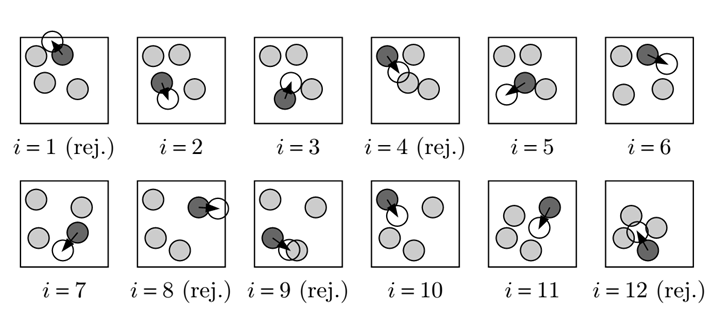
\includegraphics[scale=0.4]{mcm.png}
	\caption{Ilustração do algoritmo da cadeia de Markov.
	\label{mcm}}
\end{figure}

Implementando o algoritmo acima obtemos os resultados mostrados nas figuras \ref{mcm1}, \ref{mcm2}, \ref{mcm3} e \ref{mcm4}.

\begin{figure}[!h]
	\centering
	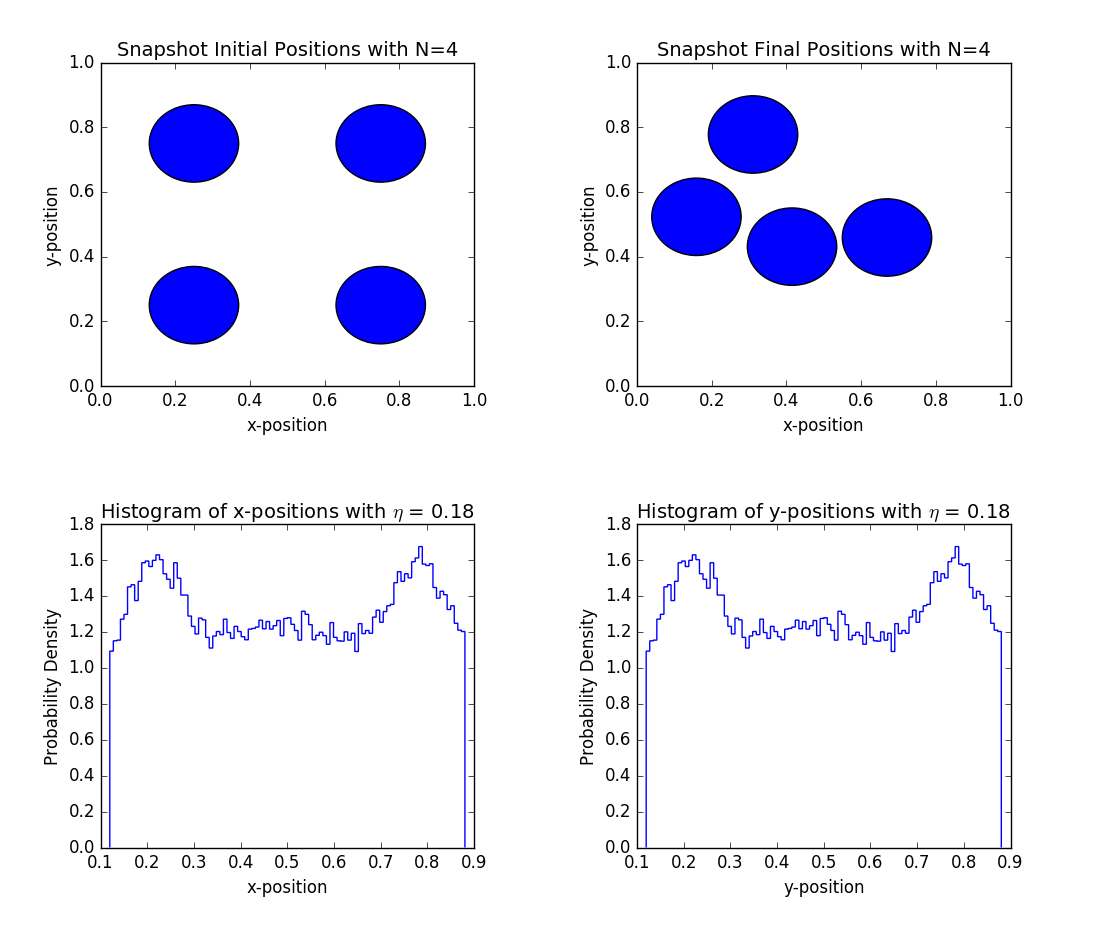
\includegraphics[scale=0.23]{mcm1.png}
	\caption{Resultado para uma simulação com rotina de $ 10^5 $ e $ \eta = 0.18 $ temos um tempo total de simulação de 1.3 segundos.
		\label{mcm1}}
\end{figure}
\begin{figure}[!h]
	\centering
	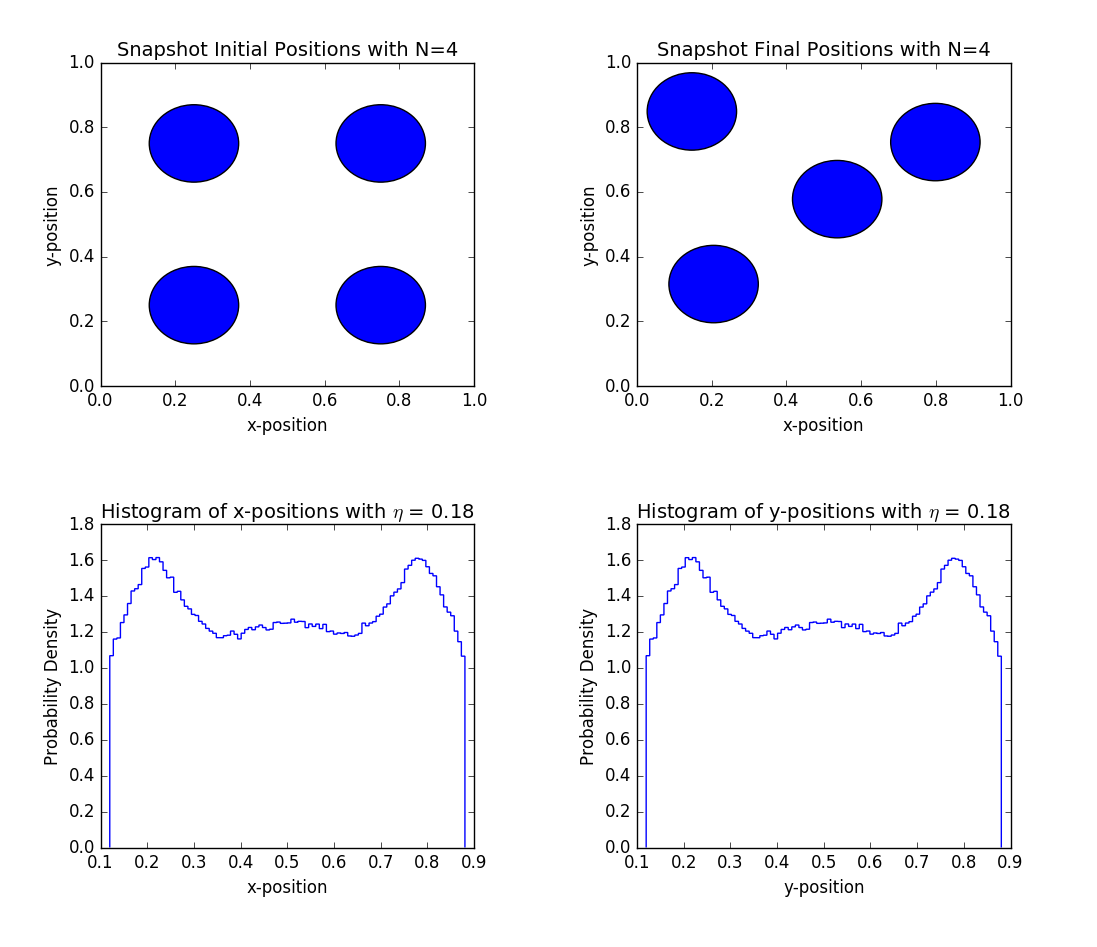
\includegraphics[scale=0.23]{mcm2.png}
	\caption{Resultado para uma simulação com rotina de $ 10^6 $ e $ \eta = 0.18 $ temos um tempo total de simulação de 6.4 segundos.
		\label{mcm2}}
\end{figure}
\begin{figure}[!h]
	\centering
	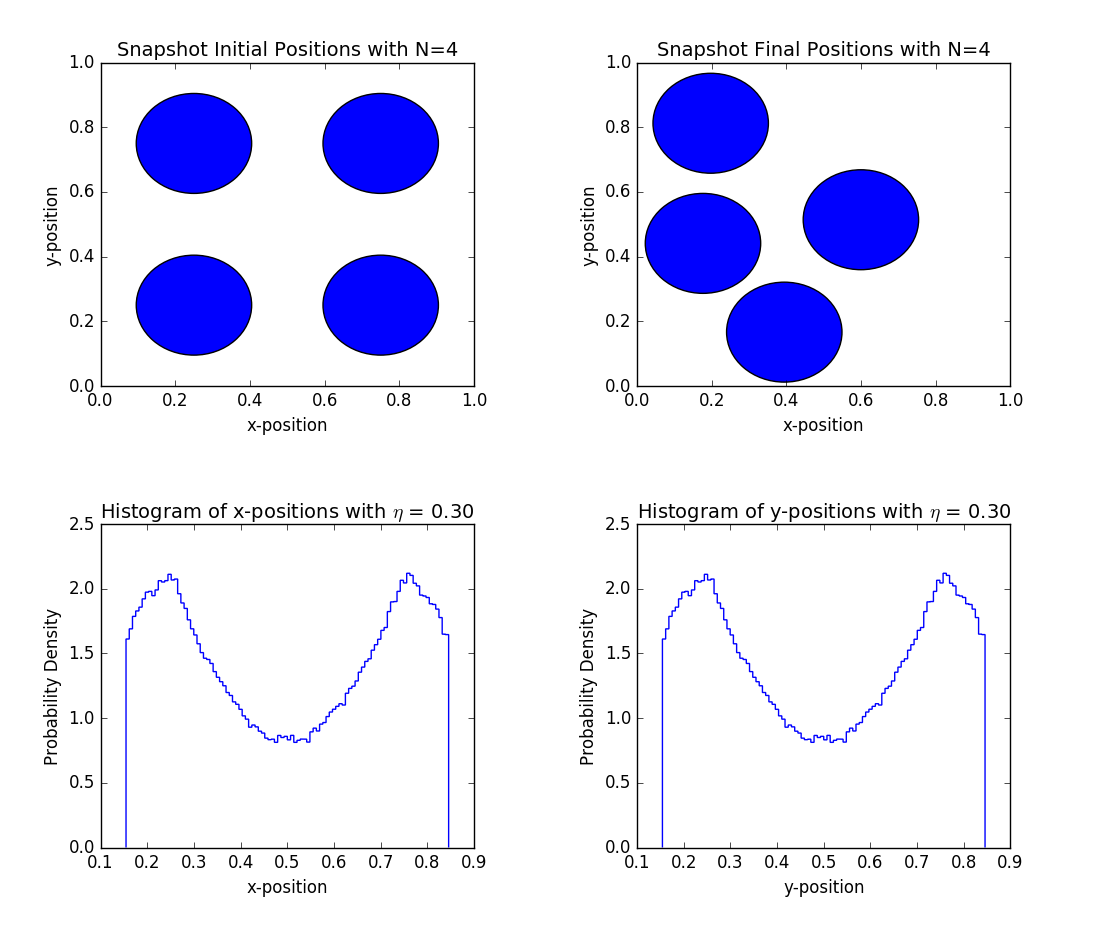
\includegraphics[scale=0.25]{mcm3.png}
	\caption{Resultado para uma simulação com rotina de $ 10^6 $ e $ \eta = 0.30 $ temos um tempo total de simulação de 6.1 segundos.
		\label{mcm3}}
\end{figure}
\begin{figure}[!h]
	\centering
	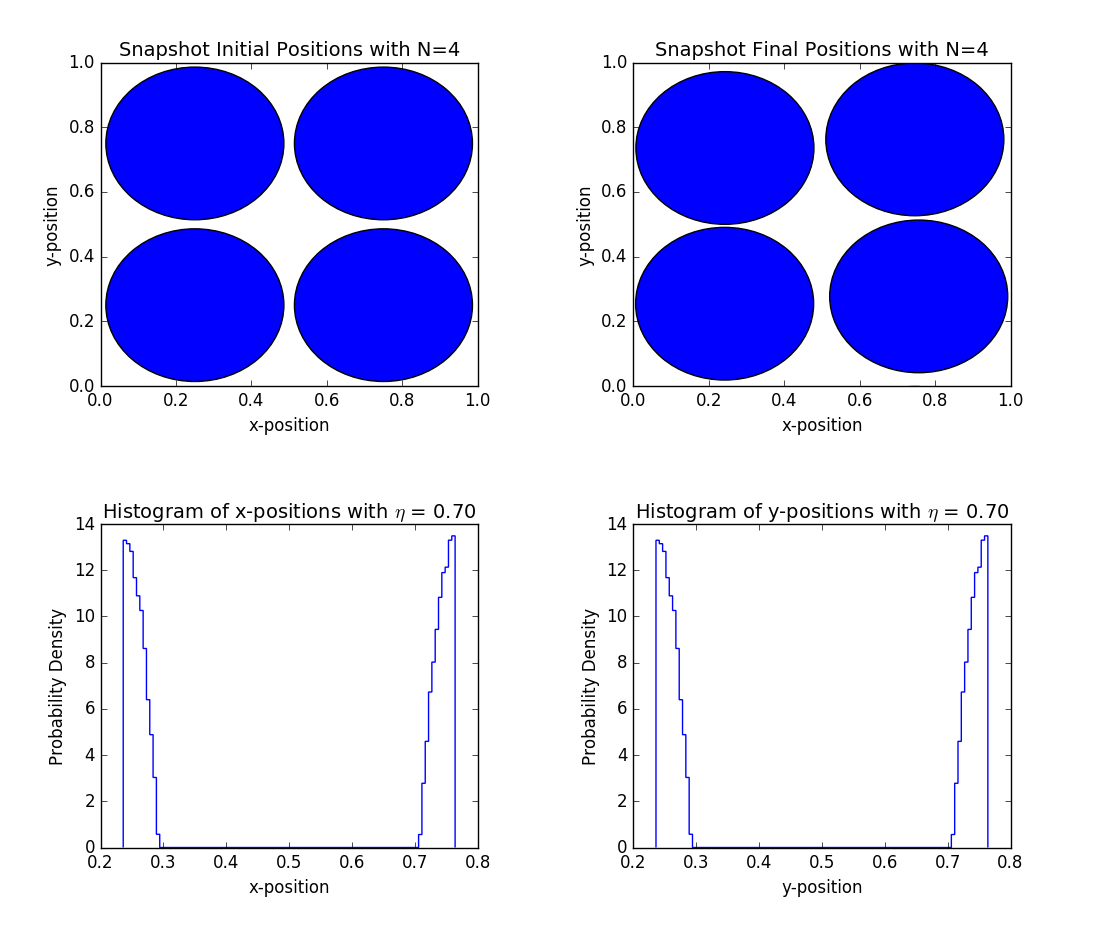
\includegraphics[scale=0.26]{mcm4.png}
	\caption{Resultado para uma simulação com rotina de $ 10^6 $ e $ \eta = 0.70 $ temos um tempo total de simulação de 5.8 segundos.
		\label{mcm4}}
\end{figure}

\newpage
Ao compararmos os resultados das figuras \ref{mcm1} e \ref{mcm2}, observamos um pequeno aumento no tempo de simulação ao aumentarmos a rotina em uma ordem de grandeza. Ao compararmos os resultados das figuras \ref{mcm2}, \ref{mcm3} e \ref{mcm4}, observamos uma constância no tempo de simulação independente do valor de $ \eta $. 

Ou seja a amostragem por cadeia de Markov é um método viável para o estudo da transição de fase que queremos observar. Porém, ainda temos um problema com o histograma de posições dessa amostragem, pois como podemos ver pelos gráficos, as posições próximas as bordas possuem uma maior probabilidade de ocorrência. Para eliminar este problema devemos implementar ao nosso algoritmo \textit{Condições Periódicas de Contorno}.

\subsection{Condições Periódicas de Contorno}

A condição periódica de contorno é utilizada com o objetivo de resolver dois grandes problemas: eliminar efeitos de superfície (as partículas que estariam na superfície sofrem efeitos como se estivessem no interior de um sistema) e a inviabilidade computacional de se trabalhar com um numero elevado de partículas de um sistema real. Esta técnica possibilita a realização de simulações utilizando um número relativamente pequeno de partículas.

Com aplicação das condições periódicas de contorno, a caixa de simulação possui réplicas idênticas em todas as direções, de modo que caso uma partícula saia por uma das faces, sua imagem entra pela face oposta, conservando assim o número total de partículas na caixa. A figura \ref{cpc} mostra um esquema das condições periódicas de contorno.

\begin{figure}[!h]
	\centering
	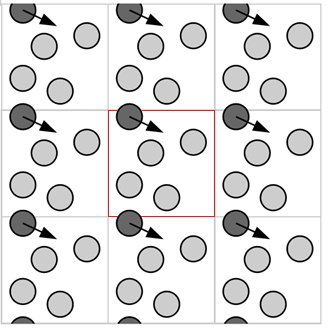
\includegraphics[scale=0.7]{cpc.png}
	\caption{Representação de um sistema com condições periódicas de contorno. As partículas podem entrar ou sair da caixa atravessando qualquer um dos lados da caixa.
		\label{cpc}}
\end{figure}

Implementando condições periódicas de contorno ao algoritmo da cadeia de Markov, obtemos os resultados mostrados nas figuras \ref*{cpc1} e \ref{cpc2}.

\begin{figure}[!h]
	\centering
	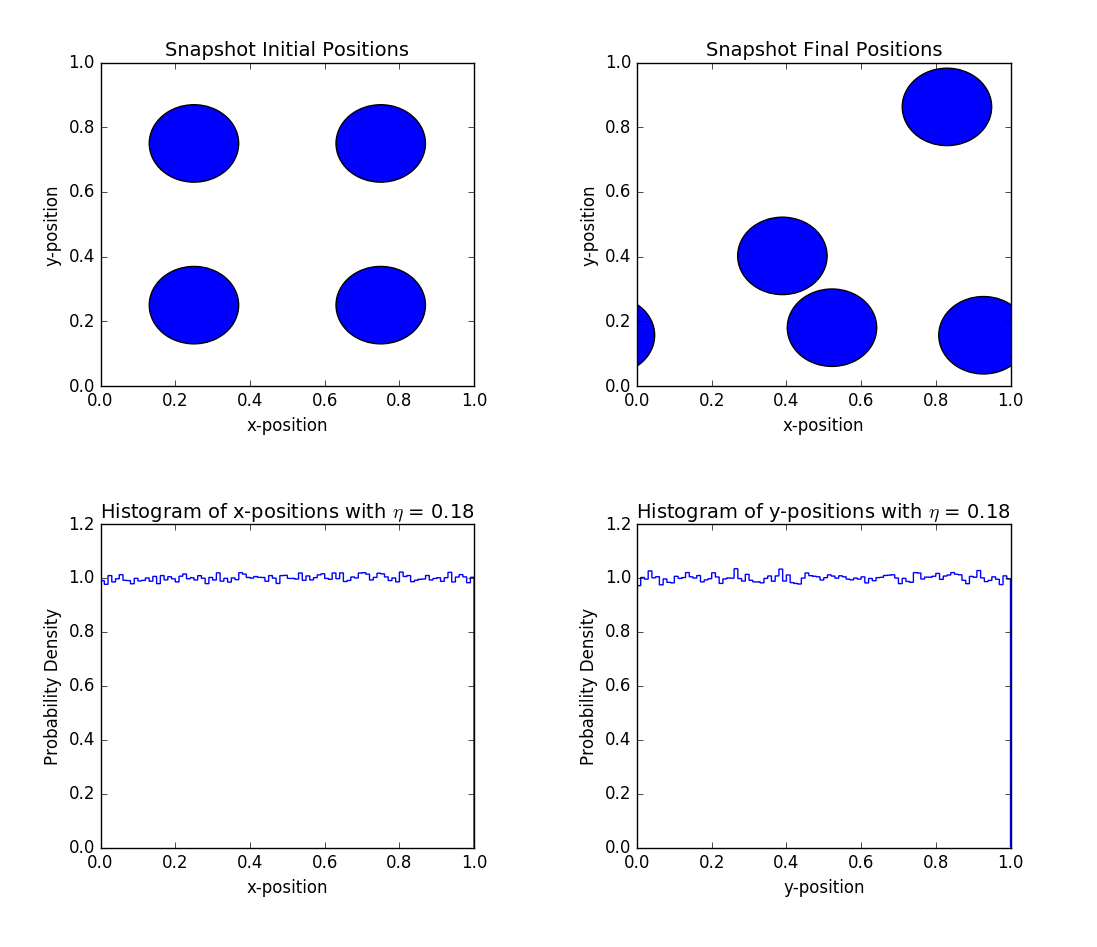
\includegraphics[scale=0.3]{cpc1.png}
	\caption{Resultado para uma simulação com rotina de $ 10^6 $ e $ \eta = 0.18 $ temos um tempo total de simulação de 7.2 segundos.
		\label{cpc1}}
\end{figure}
\clearpage
\begin{figure}[!h]
	\centering
	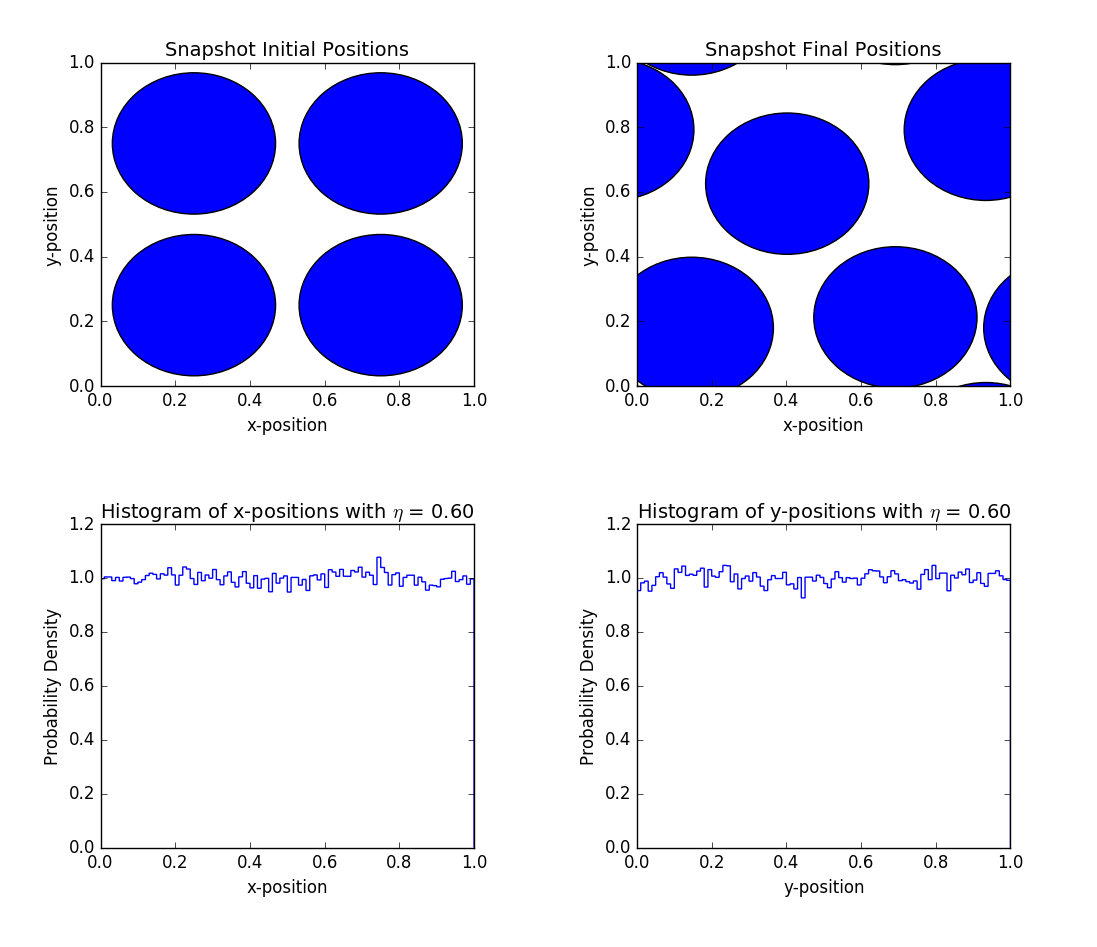
\includegraphics[scale=0.3]{cpc2.png}
	\caption{Resultado para uma simulação com rotina de $ 10^6 $ e $ \eta = 0.6 $ temos um tempo total de simulação de 7.7 segundos.
		\label{cpc2}}
\end{figure}

A partir dos resultados, observamos que todas as posições no interior da caixa possuem a mesma probabilidade de ocorrência. Logo, verifica-se que as condições periódicas de contorno foram implementadas com sucesso. Podemos então simular um sistema de muitas partículas buscando observar uma transição de fase.

\section{Amostragem cadeia de Markov para muitos discos}

Para conseguirmos explorar uma maior gama de densidades, escolhemos como configuração inicial um padrão hexagonal (figura \ref{ph}), que otimiza o valor de $ \eta $.

\begin{figure}[!h]
	\centering
	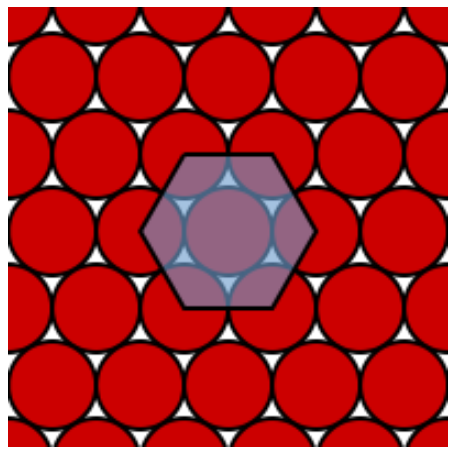
\includegraphics[scale=0.4]{ph1.png}
	\caption{Ilustração do padrão hexagonal escolhido como configuração inicial.
	\label{ph}}
\end{figure}

\newpage

Simulando o algoritmo de Markov com condições periódicas de contorno e tendo como condição inicial o padrao hexagonal, obtemos os resultados mostrados nas figuras \ref*{md055}, \ref*{md085}, \ref*{md065}, \ref*{md075}, \ref*{md068} e \ref*{md073}.

\begin{figure}[!h]
	\centering
	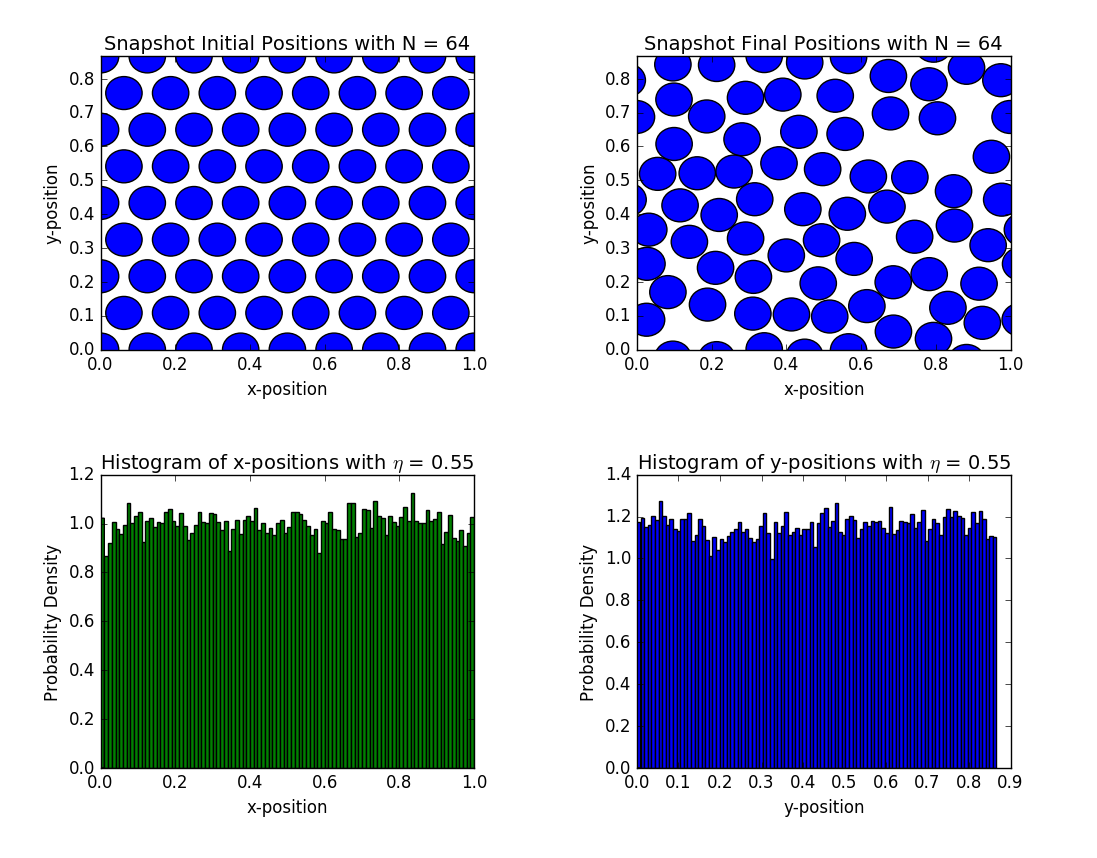
\includegraphics[scale=0.3]{md055.png}
	\caption{Resultado para uma simulação com rotina de $ 10^6 $ e $ \eta = 0.55 $.
		\label{md055}}
\end{figure}
\begin{figure}[!h]
	\centering
	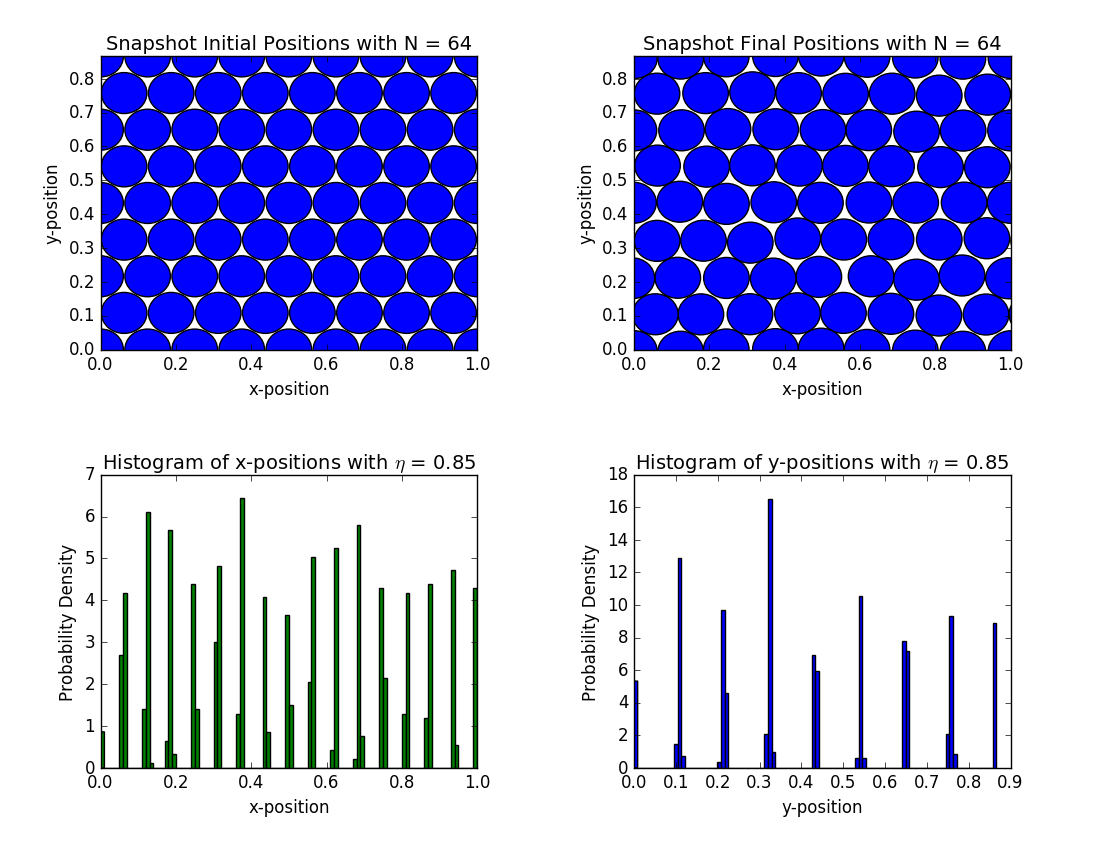
\includegraphics[scale=0.3]{md085.png}
	\caption{Resultado para uma simulação com rotina de $ 10^6 $ e $ \eta = 0.85 $.
		\label{md085}}
\end{figure}
\begin{figure}[!h]
	\centering
	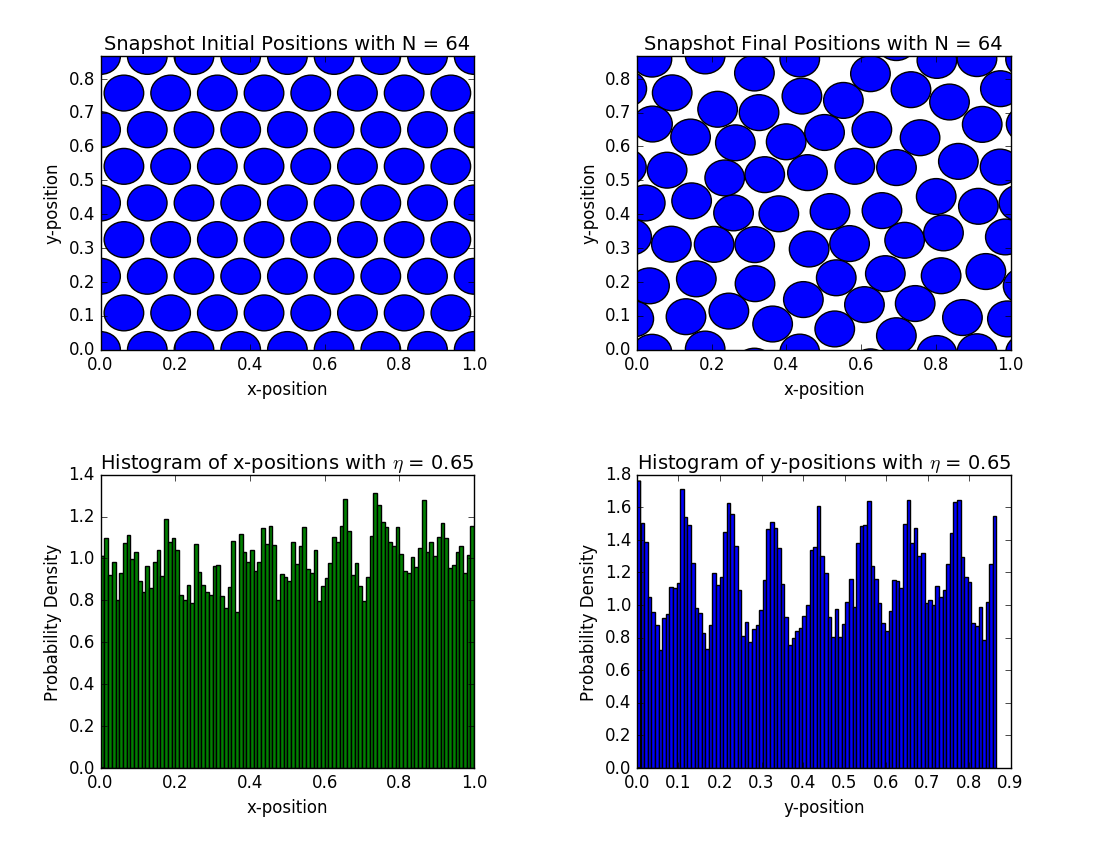
\includegraphics[scale=0.3]{md065.png}
	\caption{Resultado para uma simulação com rotina de $ 10^6 $ e $ \eta = 0.65 $.
		\label{md065}}
\end{figure}
\begin{figure}[!h]
	\centering
	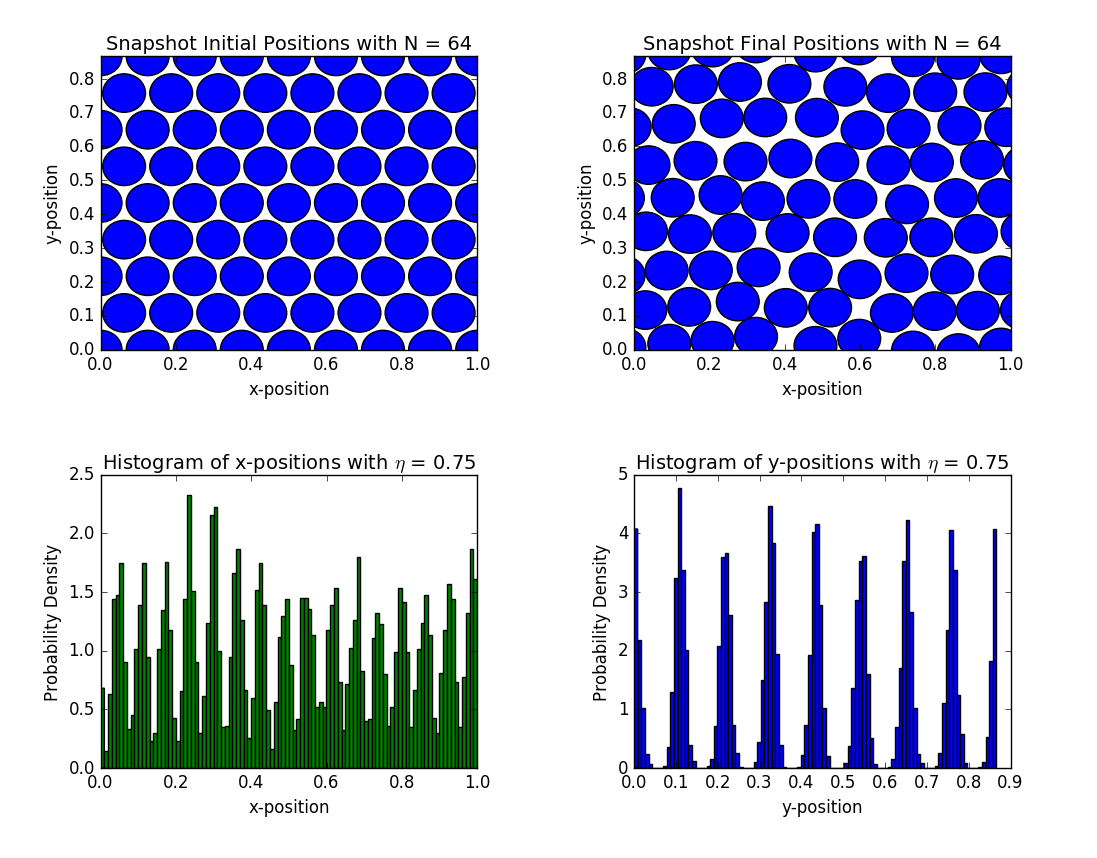
\includegraphics[scale=0.3]{md075.png}
	\caption{Resultado para uma simulação com rotina de $ 10^6 $ e $ \eta = 0.75 $.
		\label{md075}}
\end{figure}
\begin{figure}[!h]
	\centering
	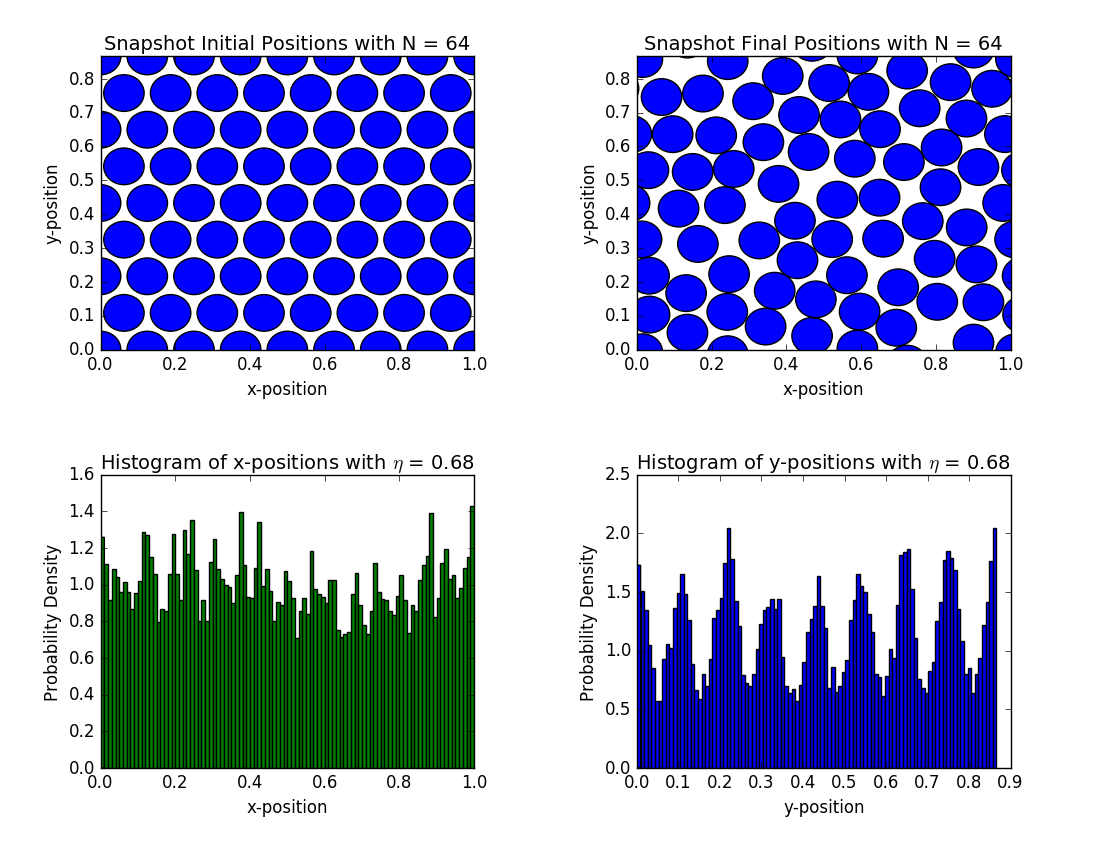
\includegraphics[scale=0.3]{md068.png}
	\caption{Resultado para uma simulação com rotina de $ 10^6 $ e $ \eta = 0.68 $.
		\label{md068}}
\end{figure}
\clearpage
\begin{figure}[!h]
	\centering
	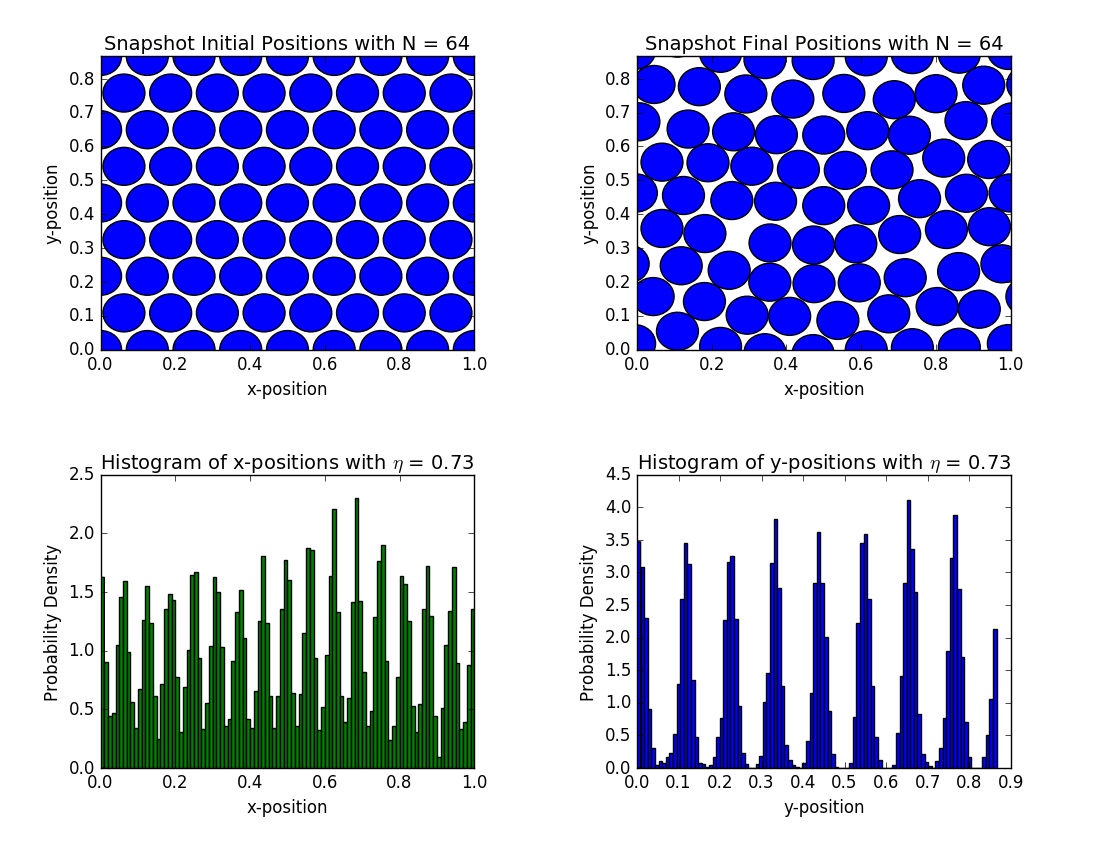
\includegraphics[scale=0.3]{md073.png}
	\caption{Resultado para uma simulação com rotina de $ 10^6 $ e $ \eta = 0.73 $.
		\label{md073}}
\end{figure}


Analisando os resultados desta simulação, podemos observar que para valores de $ \eta < 0.68$ o sistema possui uma liberdade no movimento e sua configuração inicial não é conservada, que são características típicas de amostras líquidas. Já para valores de $ \eta > 0.73 $ o sistema não possui quase nenhuma liberdade de movimentação; ademais, este movimento se dá com grande frequência nos mesmos lugares. Também podemos ver uma conservação da configuração inicial, características estas que são típicas de amostras sólidas. Portanto, nosso sistema de discos rígidos possibilitou a observação de uma transição de fase do tipo líquido-solido.


	
	%Since the photon is a transverse electromagnetic wave, it couples most strongly to the transverse optical phonons. For photon frequencies between the transverse and longitudinal optical phonon frequencies, the reflection is very high. 
	
\subsection*{Função Distribuição Radial }

Em computação científica, uma função distribuição radial, $ g(r) $, descreve como a densidade da matéria circundante varia em função de um ponto distinto. A função $ g(r) $ contabiliza a densidade local de ocorrência de vizinhos \textit{j} em torno de uma partícula \textit{i}, normalizada pela densidade do sistema. Pode-se representar esta probabilidade através de um gráfico de ocorrências (figura \ref{fdr}) em que a partícula \textit{i} esta localizada na origem, onde o eixo x define a distancia \textit{r} entre uma dada partícula \textit{j} da sua vizinha \textit{i} (figura \ref{fdr1}).

\begin{figure}[!h]
	\centering
	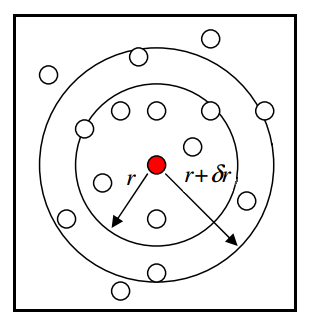
\includegraphics[scale=0.5]{fdr1.png}
	\caption{Representação de um sistema de discos rígidos, onde a distância $r$ define o raio da primeira camada de vizinhos e $ \delta r$ é definido pela distancia entre duas camadas consecutivas. O disco central em vermelho representa uma partícula \textit{i}, enquanto os pequenos discos brancos representam os vizinhos \textit{j}.
		\label{fdr1}}
\end{figure}


\begin{figure}[!h]
	\centering
	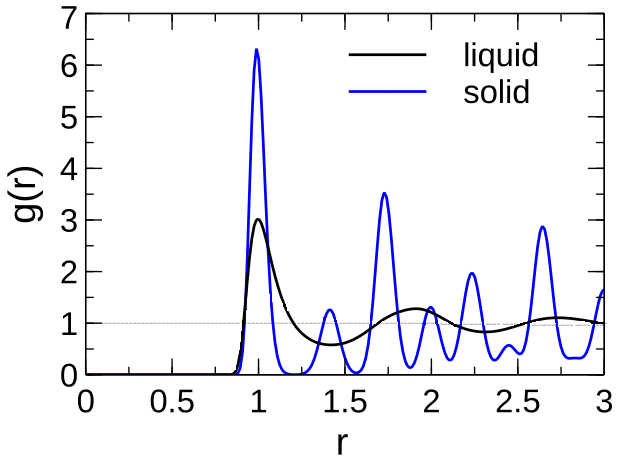
\includegraphics[scale=0.4]{fdr.png}
	\caption{Representação da função de distribuição radial para sistemas do tipo solido e líquido.
	\label{fdr}}
\end{figure}

Calculando $ g(r) $ para as densidades de transição encontradas através da simulação da cadeia de Markov com uma rotina de $ 10^6 $, obtemos os resultados mostrados nas figuras \ref{fdr068} e \ref{fdr073}.


\begin{figure}[!h]
	\centering
	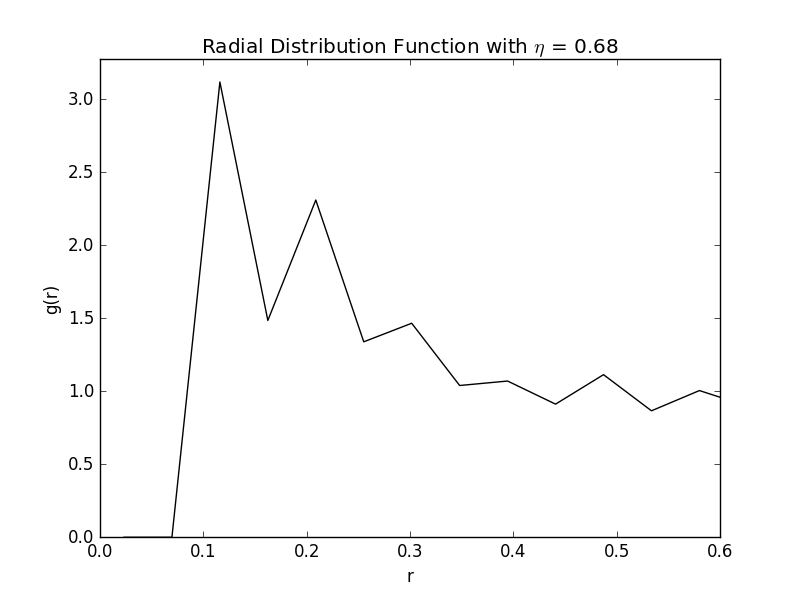
\includegraphics[scale=0.3]{fdr068.png}
	\caption{Resultado da função de distribuição radial para $ \eta = 0.68 $.
		\label{fdr068}}
\end{figure}
\begin{figure}[!h]
	\centering
	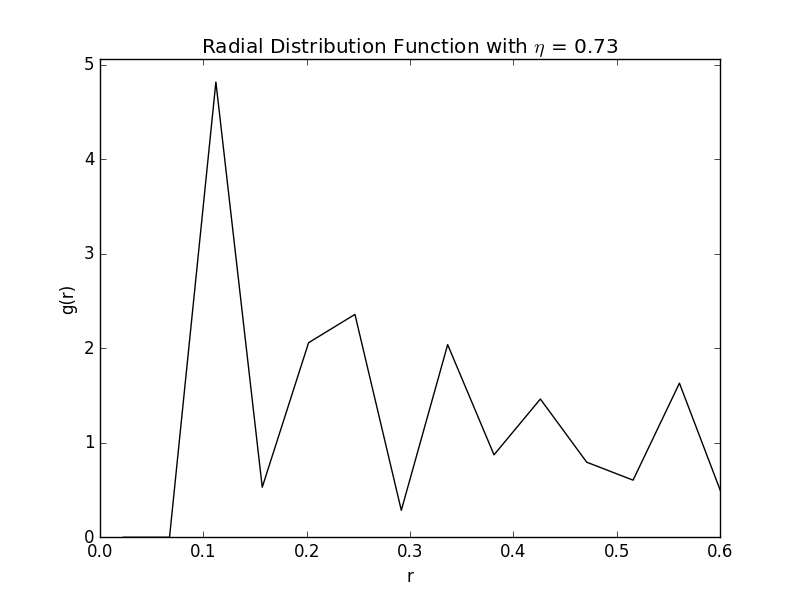
\includegraphics[scale=0.3]{fdr073.png}
	\caption{Resultado da função de distribuição radial para $ \eta = 0.73 $.
		\label{fdr073}}
\end{figure}

Analisando as figuras \ref{fdr068} e \ref{fdr073}, vemos um comportamento semelhante ao de líquido para $ \eta = 0.68 $ e de sólido para $ \eta = 0.73 $. Porém, o algoritmo que calcula $ g(r) $ ainda precisa ser melhorado para obtermos resultados mais satisfatórios.



\section{Conclusão}
Neste trabalho estudamos sistemas de discos rígidos através de simulações computacionais, implementando métodos de simulação que realizam a integração das equações de movimento de Newton e métodos estocásticos.

A \textit{Dinâmica Molecular} se mostrou um algoritmo ineficiente pois o tempo de simulação e a dificuldade de implementação crescem com a adição de novos discos ao sistema. 
O algoritmo de \textit{amostragem direta} também se mostrou ineficiente pois está restrito a simulações com um baixo número de discos e baixas densidades. A amostragem por \textit{cadeia de Markov} se mostrou um algoritmo poderoso, pois este aceita um alto número de discos e altos valores de densidade, possibilitando assim a observação uma transição de fase líquido-solido em nosso sistema. 

Para valores de $ \eta<0.68 $ temos um sistema em fase liquida e para valores de $ eta>0.73 $ temos um sistema em fase solida.


	
\section*{Agradecimentos}
		
Agradeço a CAPES pelo suporte financeiro e a Unicamp por fornecer a infraestrutura para esta pesquisa.

\section*{Referências}

\begin{enumerate}
 % retirar a numeração desta página.


\bibitem{alder}
B. J. Alder and T. E. Wainwright
\newblock \textit{"Phase Transition for Hard Sphere System".}
\newblock J. Chem. Phys. 27, 1208-1209 (1957). 


\bibitem{newman}
M. E. J. Newman and G. T. Barkema, 
\newblock \textit{"Monte Carlo Methods in Statistical Physics".}
\newblock Oxford University Press (1999).

\bibitem{metrop}
M. N. Rosenbluth, A. H. Teller, E. Teller, N. Metropolis and A. W. Rosenbluth. \newblock \textit{"Equation of State Calculations by Fast Computing Machines".}
\newblock J. Chem. Phys. 21, 1087 (1953).

\bibitem{alder2}
B. J. Alder and T. E. Wainwright
\newblock \textit{"Phase transition in elastic disks".}
\newblock J. Chem. Phys. 127, 359-361 (1962). 

\bibitem{allen}
D. J. Tildesley and M. P. Allen 
\newblock \textit{"Computer Simulation of Liquids".}
\newblock Oxford University Press (1989). 


\bibitem{mcf}
C. Scherer
\newblock \textit{"Métodos Computacionais da Física".}
\newblock Livraria da Física (2010).

\bibitem{malvin}
 M. H. Kalos, P. A. Whitlock
\newblock \textit{"Monte Carlo Methods".}
\newblock WILEY­VCH Verlag GmbH  \&  Co.KGaA  (2008).

\bibitem{krauth}
*W. Krauth
\newblock \textit{"Statistical Mechanics: Algorithms and Computations".}
\newblock Oxford University Press (2006).

\bibitem{john}
J. G. Kirkwood
\newblock \textit{"Theory of Liquids".}
\newblock Science Publishers (1968).

\bibitem{john}
*G. Ciccotti, D. Frenkel and I. R. McDonald 
\newblock \textit{"Simulation of Liquids and Solids".}
\newblock Elsevier Science Publishers (1987).



\end{enumerate}	
	
	%%%%%%%%%%%%%%%%%%%%%%%%%%%%%%%%%%%%%%%%%%%%%%%%%%%%%%%%%%%%%%%%%%%%%%%%%%%%%%%%
	
	

	
	
	
	
	
	
	
\end{document}
%
% ****** End of file apssamp.tex ******
